\chapter{Appendix - Using SuperGlue}
\label{appendix}

This appendix contains a general overview of how tags are extracted from video stories in \textit{This is How} using SuperGlue. A deeper technical overview of SuperGlue can be found in \url{https://www.pubpub.org/pub/super-glue}. This appendix requires a minimal understanding of web technologies. 

In this overview I use the \textit{Cradles to Crayons} video mentioned in \ref{video_production} as an example.

\section{Posting to SuperGlue}

The minimal requirement for submitting a video to SuperGlue is the existence of the video in a publicly accessible url. It is recommended to submit a subtitles file for text analysis although if not supplied, one will be generated using an automatic transcription algorithm. It is also recommended adding a title string and a source string for debugging purposes. 

The actual submission to SuperGlue happens through an HTTP POST request to \url{http://super-glue.media.mit/post_video} which accepts a JSON\cite{json} encoded document. 

\subsection*{Example of HTTP Post Request:}

\begin{lstlisting}[language=javascript]
{
  "title" : "Cradles to Crayons",
  "media_url": "https://dl.dropboxusercontent.com/u/3829383/c2c.mov",
  "source": "this-is-how"
}
\end{lstlisting}

The return value of this HTTP POST is also a JSON encoded document which contains a \textit{result} field. If the result is ``ok'' another field named \textit{id} will contain a generated id for this video for future reference. 

\vspace*{12pt}

\subsection*{Example of HTTP Post Response:}

\begin{lstlisting}[language=javascript]
{
  {
    "result" : "ok",
    "id": "57ba3a303c85800001d5e16a",
  }
}
\end{lstlisting}

\section{Exploring metadata using the SuperGlue Dashboard}

Upon submission of the video, a set of analysis modules will begin to analyze it. The results of all of these analyses will be stored in a publicly visible metadata document. One way to explore this document is through the SuperGlue Dashboard:

\begin{figure}[thpb]
  \centering
  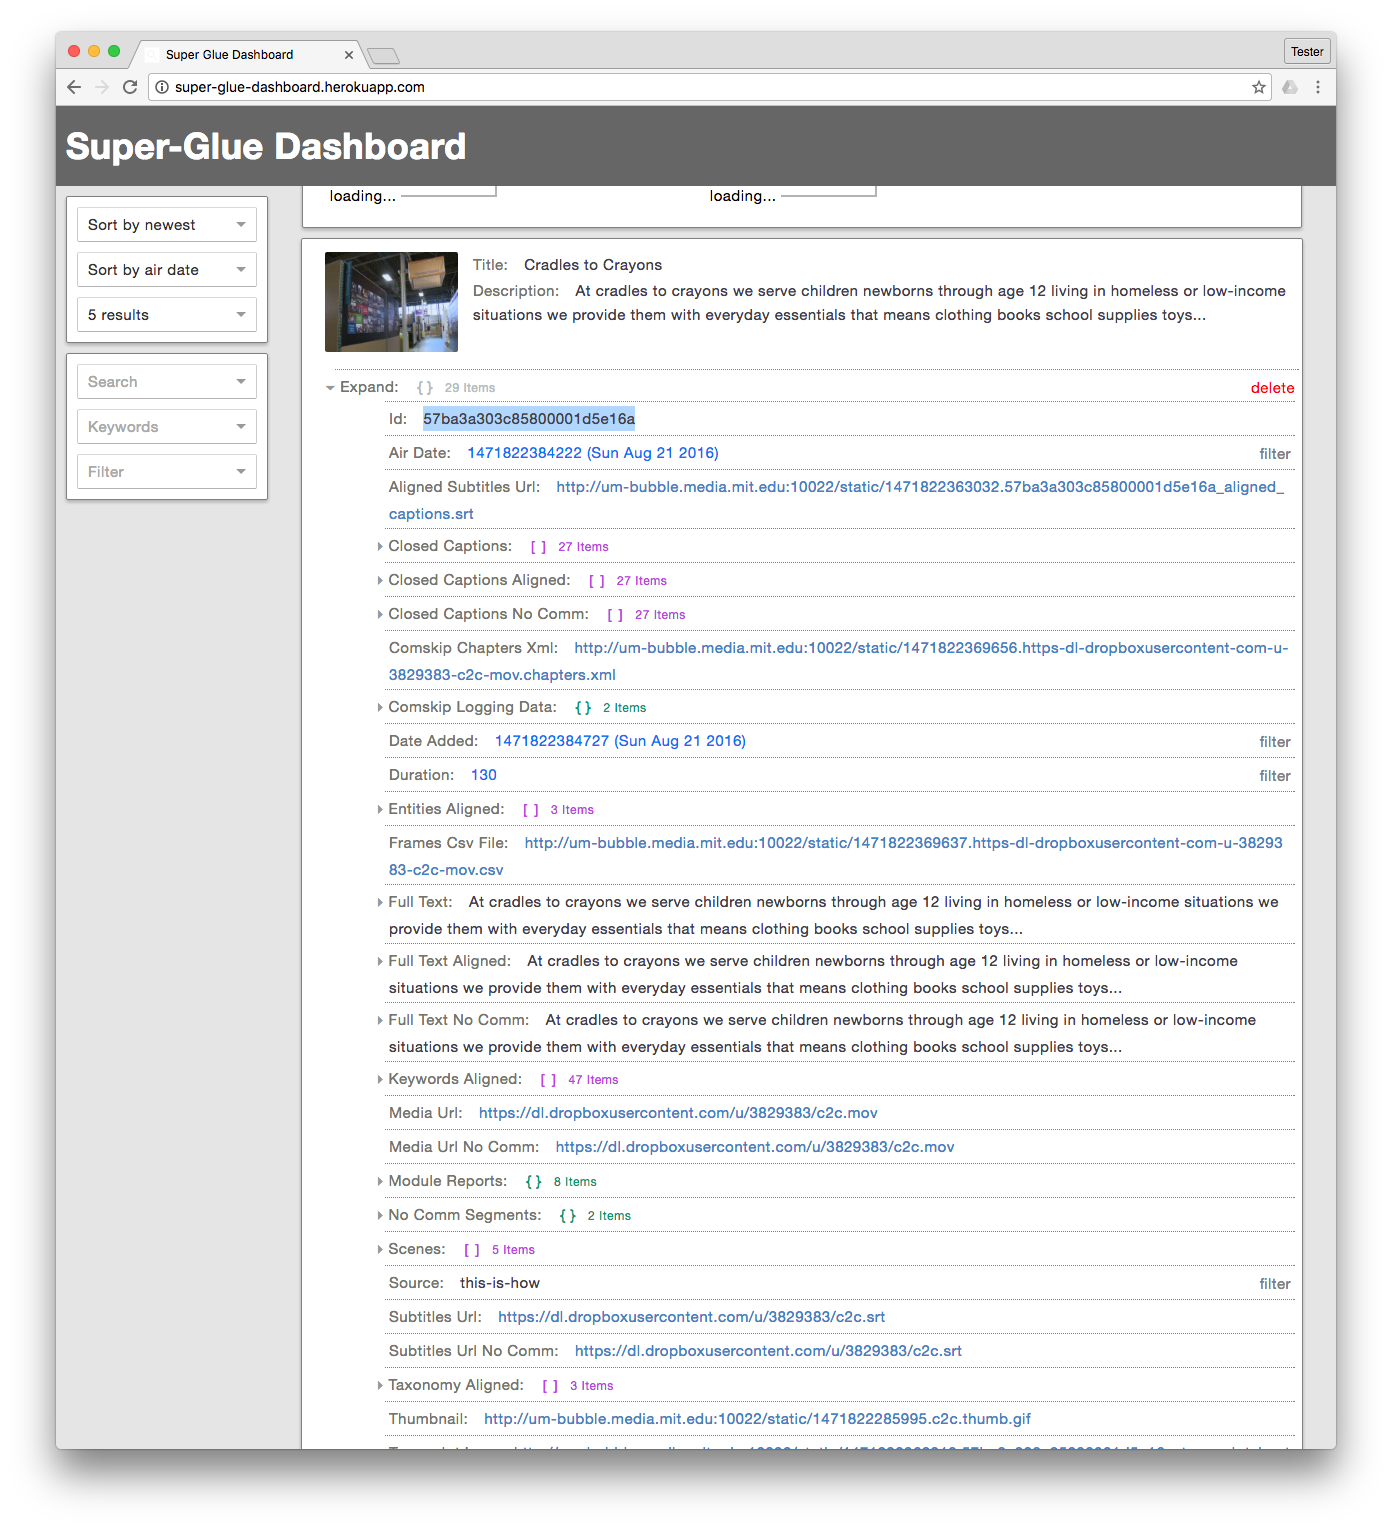
\includegraphics[width=\textwidth]{figures/super-glue-dashboard.png}
  \caption{SuperGlue dashboard displaying metadata}
  \label{fig_superglue_dashboard}
\end{figure}

Each field in the document corresponds to an analysis module. The \textit{taxonomyaligned} field contains taxonomy extracted from aligned (verified) subtitles and it will be used as our source of automatically generated tags. 

\section{Accessing metadata on SuperGlue}

There are two ways to query for metadata on SuperGlue beyond using the dashboard: a public HTTP API and direct access to the underlying mongodb\cite{mongodb} database. Direct access allows for fine tuned queries but requires working from a machine trusted by the database. The following is a mongodb query that fetches the document by the id we received in the first step and filters for taxonomy.

\subsection*{MongoDB Query:}

\begin{lstlisting}[language=javascript]
db.media.find(
  { _id : ObjectId("57ba3a303c85800001d5e16a") },
  { taxonomy_aligned : 1 })
\end{lstlisting}

\vspace*{12pt}
\subsection*{MongoDB Query Result:}

\begin{lstlisting}[language=javascript]
{
  "_id" : ObjectId("57ba3a303c85800001d5e16a"),
  "taxonomy_aligned" : [
    {
      "confident" : "no",
      "score" : "0.284283",
      "label" : "/family and parenting/children"
    },
    {
      "confident" : "no",
      "score" : "0.159685",
      "label" : "/family and parenting"
    },
    {
      "confident" : "no",
      "score" : "0.100739",
      "label" : "/shopping/toys"
    }
  ]
}
\end{lstlisting}

In \textit{This is How} tags are extracted from taxonomy labels. Per label, the most specific category is chosen and if the category contains multiple words, only the first one is chosen. 

Based on these rules the automatically generated tags for this video are \textit{children}, \textit{family} and \textit{toys}.